\chapter{Speech Recognition}
\label{chap:Speech Recognition}
Speech recognition is a sub-field of machine learning in which allows a computer program to extract and recognize words or sentences from a human being language, and converting them back to a machine language. Advance techniques nowadays, permits to understand natural speech for executing tasks. Google Voice Search\footnote{\url{https://www.google.com/search/about/}} and Siri\footnote{\url{http://www.apple.com/ios/siri/}} are two examples of very advance speech recognition softwares with the capability of understanding natural language.

\section{The Problem of Speech Recognition}
\label{sec:The Problem of Speech Recognition}
Human languages are very complex and different among each other. Despite they might have a well-structured grammar, automatically recognition is still a very difficult problem since people have many ways to say the same thing. In fact, spoken language is different from written one because the articulation of verbal utterance is less strict and complicated. \\
The environment in which the sound is taken has a big influence on the speech recognition software because it introduces a \textit{unwanted} amount of information in the signal. For this reason it is important that the system is capable of \textit{identifying} and \textit{filtering out} this surplus of information \cite{forsberg2003speech}. \\

\noindent Another interesting set of problems are related to the speaker itself. Each person has a different body that means there are a variety of components that the recognition system has to take care of in such a way to be able to understand correctly. Gender, vocal tracts, speaking style, speed of the speech, regional provenience are fundamental parts that have to be taken in consideration when building the \textit{acoustic model} for the system. Despite these features are unique for each person, there some common aspects that will be used to construct the model. The acoustic model represents the relationship between the acoustic signal of the speech and the phonemes related to it. \\

\noindent Ambiguity represents the major concern since natural languages have inherited it. In fact, it may happen that in a sentence we are not able to discriminate which words are actually intended \cite{forsberg2003speech}. In speech recognition there are two types of ambiguity: \textit{homophones} and \textit{word boundary ambiguity}. \\
Homophones refers to those words that are spelled in a different way but they \textbf{sound} the same. Generally speaking, these words are not correlated to each other but it happened that the sound is equivalent. Word boundary ambiguity instead, it \textit{occurs when there are multiple ways of grouping phones into words}\cite{forsberg2003speech}.

% CMU Sphinx4
\section{Architecture}
\label{sec:speech_rec_Architecture}
Generally speaking, a speech recognition system is divided in three main components: the \textbf{Feature Extraction} (or Front End), the \textbf{Decoder} and the \textbf{Knowledge Base} (KB). In \ref{fig:speech_architecture} the KB part is represented by the three sub-blocks called \textit{Acoustic Model}, \textit{Pronunciation Dictionary} and \textit{Language Model}. The \textit{Front End} takes as in input the voice signal where it is analyzed and converted in the so called \textit{Features Vectors}. This last is the set of common properties that we discussed in \ref{ch:english_language}. From here we can say that $\textbf{Y} 1:N = y_{1},..., y_{N}$ where $Y$ is the set of features vectors. \\
The second step consists in feeding the \textit{Decoder} with vectors we obtained from the previous step, attempting to find the sequence of words $\textbf{w} 1:L = w_{1}, ... , w_{L}$ that have most likely generated the set $Y$\cite{gales2008application}. The decoder tries to find the likelihood estimation as follows:

\begin{equation}
	\widehat{w} = \underset{w}{arg \, max} \,\, P(\textbf{w}| \textbf{Y})
\end{equation} 

\noindent The $P (w|Y)$ is difficult to find directly\footnote{There is discriminate way of finding the estimation directly as described in \cite{gales2007discriminative}}, but using Bayes' Rules we can transform the equation above in

\begin{equation}
	\widehat{w} = \underset{w}{arg \, max} \,\, P (\textbf{Y}|\textbf{w}) P(\textbf{w})
\end{equation}

\noindent in which the probability $P(Y|w)$ and $P(w)$ are estimated by the \textit{Knowledge Base} block. In particular, the \textit{Acoustic Model} is responsible to estimate the first one whereas the \textit{Language Model} estimates the second one. \\
\noindent Each word \textbf{w} is decomposed in smaller components called \textit{phones}, representing the collection of phonemes $\textbf{K}_{w}$ (see \ref{ch:english_language}). We can describe the \textit{pronunciation} as $\overset{(w)}{\textbf{q}_{1:K_{w}}} = q_{1}, ...., q_{K_{w}}$. The likelihood estimation of the sequence of phonemes is calculated by a \textbf{Hidden Markov Model} (HMM). In the section, a general overview of HMM is given. We are not going to discuss a particular model because every speech recognition system uses a variation of the general HMM chain. \\

\begin{figure}[!ht]
	\centering
	\includegraphics[scale=0.8]{Figures/speech_Architecture.png}
	\caption{HMM-Based speech recognition system \cite{gales2008application}}
	\label{fig:speech_architecture}
\end{figure}

\section{Hidden Markov Model}
\label{sec:hmm}
\noindent A definition given by \cite{eddy1996hidden} is the following: \textit{"An Hidden Markov Model is a finite model that describes the probability distribution over an infinite number of possible sequences"}. Each sequence is determined by a set of \textit{transition probabilities} in which describes the transitions among states. The \textbf{observation} (or outcome) of each state is generated based on the associated probability distribution. From an \textit{outside} perspective, the \textit{observer} is only able to see the outcome and not the state itself. Hence, the states are considered \textbf{hidden} which leads to the name Hidden Markov Model \cite{def_hmm}. \\

\noindent An HMM is composed by the following elements:

\begin{itemize}
	\item The number of states (N)
	\item The number of observations (M), that becomes infinite if the set of observations is contiguous
	\item The set of transition probabilities, $\Lambda = \{ a_{ij}\}$
\end{itemize}

The set of probabilities is defined as follow:
\begin{equation}
\label{eq:transition_probabilities}
a_{ij} = p \, \{ \, q_{t+1} = j \, | \, q_{t} = i \, \}, \, \, \, 1 \leq i,j \leq N, 
\end{equation}

\noindent where $q_{t}$ is the state we are currently in and $a_{ij}$ represent the transition from state $i$ to $j$. 
Each transition should satisfy the following rules:

\begin{subequations}
	\label{eq:stochastic_rules}
	\begin{align}
	a_{ij} \geq 1, \, \, \, 1 \leq i,j \leq N, \\
	\sum_{j=1}^{N} a_{ij} = 1, \, \, \, 1 \leq j \leq N
	\end{align}
\end{subequations}

\noindent For each state $S$ we can define the probability distribution $S = \{s_{j}(k)\}$ as follow:

\begin{equation}
s_{j}(k) = p \, \{\, o_{t} = v_{k} \, | \, q_{t} = j \, \}, \, \, \, 1 \leq j \leq N, \,\, 1 \leq k \leq M
\end{equation}

\noindent where $v_k$ is the $k^{th}$ observation whereas $o_{t}$ is the outcome. Furthermore, $b_{j}(k)$ must satisfy the same stochastic rules described in \ref{eq:stochastic_rules}. \\

\noindent A different approach is made when the number of observations is infinite. In fact, we are not going to use a set of discrete probabilities but instead a continuous probability density function. Given that, we can define the parameters of the density function by approximating it by a weighted sum of $M$ Gaussian distributions $\varphi$ \cite{def_hmm}. We can describe the function as follow:

\begin{equation}
	s_{j}(o) = \sum_{m = 1}^{M} c_{jm}\varphi (\mu_{jm}, \Sigma_{jm}, o_{t})
\end{equation}

\noindent where $c_{jm}$ is the weighted coefficients, $\mu_{jm}$ is the mean vector and $\Sigma_{jm}$ is the covariance matrix. The coefficients should satisfy the stochastic rules in \ref{eq:stochastic_rules}. \\
\noindent We can then define the initial state distribution as $\pi = \{\pi_{i}\}$ where 

\begin{equation}
	\pi_{i} = p \, \{ q_{I} = i \, \}, \,\,\,\, 1 \leq i \leq N
\end{equation} 

\noindent Hence, to describe the HMM with the discrete probability function we can use the following compact form
\begin{equation}
\label{eq:hmm_discrete}
	\lambda = (\Lambda, S, \pi )
\end{equation}

\noindent whereas to denote the model with a continuous density function, we use the one described in \ref{eq:hmm_density}
\begin{equation}
\label{eq:hmm_density}
\lambda = (\Lambda, c_{jm}, \mu_{jm}, \Sigma_{jm}, \pi )
\end{equation} 

\subsection{Assumptions}
\label{sub:assumptions_hmm}
The theory behind HMM requires three important assumptions: the \textbf{Markov assumption}, the \textbf{stationarity assumption} and the \textbf{output independence assumption}.

\subsubsection{The Markov Assumption}
The Markov assumption assumes that the following state depends only from the state we are currently in as given in \ref{eq:transition_probabilities}. The result model is also referred as \textit{first order} HMM. Generally speaking though, the decision of the next coming state might depend on \textbf{n} previous states, leading to a $n^{th}$ HMM order model. In this case, the transition probabilities is defined as follow:

\begin{equation}
\label{eq:transition_nth_order}
a_{i_{1}i_{2}...i_{n}j} = p\, \{\, q_{t+1} = j \,|\, q_{t} = i_{1}, \, q_{t-1} = i_{2}, ... , \, q_{t-k+1} = i_{k} \, \}, \,\,\,\, 1 \leq i_{1},i_{2}, ... ,i_{k}, j \leq N
\end{equation}


\subsubsection{The Stationary Assumption}
The second assumption states that the transition probabilities are \textit{time-independent} when the transitions occur. This is defined by the following equation for any $t_{1}$ and $t_{2}$:

\begin{equation}
	p \, \{\, q_{t+1} = j \,|\, q_{t_{1}} = i\, \}\, = \,p \,\{\, q_{t_{2}+1} = j \,|\, q_{t_{2}} = i\, \}
\end{equation}

\subsubsection{The Output Assumption}
The last assumption says that the current observation is statistically independent from the previous observations. Let's consider the following observations:

\begin{equation}
	O = o_{1}, o_{2}, ... , o_{T}
\end{equation}

Now, recalling \ref{eq:hmm_discrete}, it is possible to formulate the assumption as follow:

\begin{equation}
\label{eq:final_hmm}
	p \, \{\, O \, |\, q_{1},q_{2}, ... , q_{T}, \lambda \,\}\, = \, \prod_{t = 1}^{T} p \, \{ \, o_{t} \, | \, q_{t}, \, \lambda \,\}
\end{equation}

\section{Evaluation}
The next step in the HMM algorithm is the \textit{evaluation}. This phase consists in estimating the likelihood probability of a model when it produces that output sequence. Generally speaking, there are two famous algorithms that have been extensively used: \textbf{forward} and \textbf{backward} probability algorithms. In the next two subsections, we report the two algorithms that either one can be used.

\subsection{Forward probability algorithm}
Let us consider the equation \ref{eq:final_hmm} where the probabilistic output estimation is given. The major drawback of this equation is that the computational cost is exponential in $T$ because the probability of $O$ is calculated directly. It is possible to improve the previous approach by \textit{caching} the calculations. The cache is made using a \textit{lattice} (or trellis) of states where at each time step, the $\alpha$ value is calculated by summing all the states at the previous time step \cite{hmm_tutorial}. \\

\noindent The $\alpha$ value (or forward probability) can be calculated as follow:

\begin{equation}
\label{eq:alpha_equation}
	\alpha_{t}(i) \, = \, P(o_{1}, o_{2}, ... , o_{t}, q_{t} = s_{i} | \lambda)
\end{equation}

\noindent where $s_{i}$ is the state at time $t$. \\
Given that, we can define the forward algorithm in three steps as follow:

\begin{itemize}
	\item[1.]{Initialization:} \\
		\begin{equation}
			\alpha_{1}(i) = \pi_{i}b_{i}(o_{1}), 1 \leq i \leq N
		\end{equation}		
	\item[2.]{Induction step:} \\
		\begin{equation}
		\label{eq:induction_step_forward}
			\left ( \sum_{i=1}^{N} \alpha_{t}(i) a_{ij} \right ) b_{j}(o_{t+1}) \,\, where \,\, 1 \leq t \leq T - 1, \,\, 1 \leq j \, N
		\end{equation}		
	\item[3.]{Termination:} \\
		\begin{equation}
			P(O|\lambda) = \sum_{i=1}^{N} \, \alpha_{T}(i)
		\end{equation}
\end{itemize}
		
\noindent The key of this algorithm stays in \ref{eq:induction_step_forward} where for each state $s_{j}$ the $\alpha$ value contains the probability of the observed sequence from the beginning to time $t$. Given the previous algorithm, we can now calculate the new complexity. The direct algorithm has a complexity of $2TN^{T}$ whereas the new one is $N^{2}T$.

\subsection{Backward probability algorithm}
This algorithm is very similar to the previous one with the only difference when calculating the probability. Instead of estimating the probability as in \ref{eq:alpha_equation}, the backward algorithm estimates the likelihood of \textit{"the partial observation sequence from $t+1$ to $T$, starting from state $s_{i}$"}\cite{hmm_tutorial}. \\

\noindent The probability is calculated with the following equation:

\begin{equation}
\label{eq:backward_algorithm}
	\beta_{t}(i) \, = \, P(o_{t+1}, o_{t+2}, ... , o_{T} \, | \, q_{t} = s_{i}, \, \lambda)
\end{equation}

\noindent The usage of either one depends on the type of problem we need to face.


\section{Viterbi algorithm}
\label{sec:viterbi}
The main goal of this algorithm is to discover the sequence of hidden states that are more likely to be produces given a sequence of observations. This block is called \textbf{decoder} (see \ref{fig:speech_architecture} for reference). The \textit{Viterbi algorithm} is one of the most used solution for finding a \textit{single best sequence} for a given set of observations \cite{hmm_tutorial}. What makes this algorithm suitable for this problem, is the similarity with the forwarding algorithm with the only difference that instead of summing the transition probabilities at each step, it calculates the \textbf{maximum}. In \ref{fig:hmm_recursion} it is shown how the maximization estimation is calculated during the recursion step.

\begin{figure}[!ht]
	\centering
	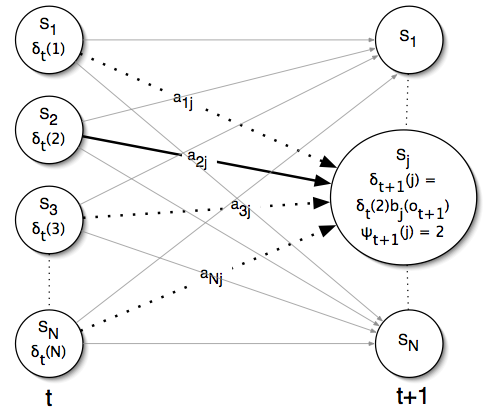
\includegraphics[scale=0.8]{Figures/hmm_recursion.png}
	\caption{The recursion step \cite{hmm_tutorial}}
	\label{fig:hmm_recursion}
\end{figure}

\noindent Let's define the probability of the most likely sequence for a given partial observation: 

\begin{equation}
	\delta_{t}(i) =  \underset{q_{1},q_{2}, ... , q_{t-1}}{\mathrm{max}} P (q_{1},q_{2}, ... , q_{t} = s_{i}, o_{1}, o_{2}, ... , o_{t} \, | \, \lambda)
\end{equation}

\noindent From here, we can define the steps of the algorithm as follow:

\begin{itemize}
	\item[1.]{Initialization:} \\
	\begin{equation}
		\delta_{1}(i) = \pi_{i}b_{i}(o_{1}), \,\, 1 \leq i \leq N, \phi_{1}(i) = 0
	\end{equation}		

	\item[2.]{Recursion:} \\
	\begin{subequations}
		\begin{align}
		\delta_{t}(j) = \underset{1\leq i \leq N}{\mathrm{max}} [\delta_{t-1}(i)a_{ij}] \, b_{j}(o_{t}), \,\, 2 \leq t \leq T, \,\, 1 \leq j \leq N, \\
		\psi_{t}(j) = \underset{1\leq i \leq N}{\mathrm{arg \, max}} [\delta_{t-1}(i)a_{ij}], \,\, 2 \leq t \leq T, \,\, 1 \leq j \leq N,
		\end{align}
	\end{subequations}		

	\item[3.]{Termination:} \\
	\begin{subequations}
		\begin{align}
		P^{*} = \underset{1\leq i \leq N}{\mathrm{max}}[\delta_{T}(i)] \\
		q_{t}^{*} = \underset{1\leq i \leq N}{\mathrm{arg \, max}}[\delta_{T}(i)]
		\end{align}
	\end{subequations}

	\item[4.]{Backtracking:} \\
	\begin{equation}
		q_{t}^{*} = \psi_{t+1}(q_{t+1}^{*}), \,\, t = T - 1, T - 2, ... , 1
	\end{equation}
\end{itemize}

\noindent As previously stated, the Viterbi algorithm maximizes the probability during the recursion step. After that, the resulting state is used as a \textit{back-pointer} in which during the backtracking step, the best sequence will be found. In \ref{fig:hmm_backtrack} is depicted how the backtracking step works.

\begin{figure}[!ht]
	\centering
	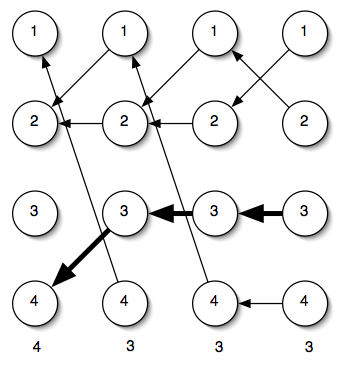
\includegraphics[scale=0.8]{Figures/hmm_backtrack.png}
	\caption{The backtracking step \cite{hmm_tutorial}}
	\label{fig:hmm_backtrack}
\end{figure}


\section{Maximum likelihood estimation}
\label{sec:mle}
The last part of the model is represented by the \textit{Learning} phase, in which the system is able to decide what it the final word pronounced by a user. With the usage of HMM models, it is possible to extract one or more sequences of states. The last piece of the puzzle is to estimate the sequence of words. To do so, a typical speech recognition system uses the \textit{Maximum Likelihood estimation} (MLE). \\

\noindent Given a sequence of $n$ \textit{independent} and \textit{identical} observations $x_{1}, x_{2}, ... , x_{n}$. Assuming that the set of samples comes from a probability distribution with an \textit{unknown density function} called $f_{0}(x_{1}, ... , x_{n})$. The function belongs to a family of a certain kind of distributions in which $\theta$ is the \textit{parameters vector} for that specific family. \\

\noindent Before using MLE, a \textit{joint density function} must be specified first for all observations. Given the previous set of observation, the joint density function can be denoted as follow:

\begin{equation}
	f (x_{1}, x_{2}, ... , x_{n} | \theta) = f(x_{1} | \theta) \times f(x_{2} | \theta) \times ... \times f(x_{n} | \theta)
\end{equation}

\noindent Now, consider the same set of observations as a \textit{fixed} parameters whereas $\theta$ is allowed to change without any constraint. From now on, this function will be called \textbf{likelihood} and denoted as follow:

\begin{equation}
	L(\theta \, \sim \, x_{1}, x_{2}, ... , x_{n}) = f (x_{1}, x_{2}, ... , x_{n} | \theta) = \prod_{i=1}^{n} f (x_{i} | \theta)
\end{equation}

\noindent In this case, $\sim$ indicates a simple separation between the parameters function and the set of observations. \\
\noindent Often, there is a need to use the \textit{log} function; that is transform the likelihood as follow:

\begin{equation}
\label{eq:log-likelihood}
	ln \, L(\theta \, \sim \, x_{1}, x_{2}, ... , x_{n}) = \sum_{i=1}^{n} ln \, f(x_{i} | \theta)
\end{equation}

\noindent To estimate the log-likelihood of a single observation, it is necessary to calculate the average of \ref{eq:log-likelihood} as follow:

\begin{equation}
\label{eq:avg-likelihood}
	\hat{l} = \frac{1}{n} ln \, L
\end{equation} 

\noindent The \textit{hat} in \ref{eq:avg-likelihood} indicates that the function is an estimator. From here we can define the actual MLE.
This method estimates the $\theta_{0}$ by finding the value of $\theta$ that returns the maximum value of $\hat{l}(\theta \, \sim \, x)$. The estimation is defined as follow if the maximum exists:

\begin{equation}
	\hat{\theta}_{mle} \subseteq \{ \underset{\theta}{arg \, max} \,\, \hat{l} \,\, (\theta \, \sim \, x_{1}, x_{2}, ... , x_{n})\}
\end{equation}

\noindent The MLE corresponds to the so called \textit{maximum a posteriori estimation} (MPE) of \textit{Bayes rule} when a uniformed prior distribution is given. In fact, $\theta$ is the MPE that maximize the probability. Given the Bayes' theorem we have:

\begin{equation}
	P (\theta | x_{1}, x_{2}, ... , x_{n}) = \frac{f(x_{1}, x_{2}, ... , x_{n} | \theta) P(\theta)}{P(x_{1}, x_{2}, ... , x_{n})}
\end{equation}

\noindent where $P(\theta)$ is the prior distribution whereas $P(x_{1}, x_{2}, ... , x_{n})$ is the averaged probability of all parameters. Due to the fact that the denominator of the Bayes' theorem is independent from $\theta$, the estimation id obtained by maximizing $f(x_{1}, x_{2}, ... , x_{n} | \theta) P(\theta)$ with respect of $\theta$.


% GMM classifier
\section{Gaussian Mixture Model}
%\label{sec:gmm}
A Gaussian mixture model is a probabilistic model where the it is assumed that the set of points come from a \textit{mixture model}, in particular from a fixed number of \textit{Gaussian distributions} where the parameters are \textit{unknown}. This approach can be thought of a generalization of the clustering algorithm called \textit{k-means} where we are looking for the \textbf{covariance} and the center of the Gaussian distribution and not only the centroids \cite{sklearn_gmm}. There are different way for fitting the mixture model, but we are going to focus in particular to the one where the expectation-maximization is involved (see \ref{sec:mle}). \\

\noindent Let the following equation defining a weighted sum of N Gaussian densities component:

\begin{equation}
	p(\textbf{x}|\lambda) = \sum_{i=1}^{N} w_{i} \, g(\textbf{x}|\mu_{i}, \Sigma_{i})
\end{equation}

\noindent where \textbf{x} defines the set of features (data-vector) of continuous values. The sequence $w_{i} = 1, ... , N$ represents the set of mixture weights whereas the function $g(\textbf{x}|\mu_{i}, \Sigma_{i}), \, i = 1, ... , N$ defines the Gaussian densities component. The following equation specifies each Gaussian component's form:

\begin{equation}
	g(\textbf{x}|\mu_{i}, \Sigma_{i}) = \frac{1}{(2\pi)^{D/2} \, |\Sigma_{i}|^{1/2}} exp \left \{ -\frac{1}{2} (\textbf{x} - \mathbf{\mu_{i}})' \,\, \Sigma_{i}^{-1} \,\, (x - \mathbf{\mu_{i}}) \right \}
\end{equation} 

\noindent where $\mathbf{\mu_{i}}$ is the mean vector and $\Sigma_{i}$ is the covariance matrix. Given that, we can assume that the mixture satisfy the constrain that $\Sigma_{i=1}^{N} \,\, w_{i} = 1$. \\

\noindent With the notation in \ref{eq:gmm}, we can now define the complete GMM since all the component densities are parameterize by the covariance matrices, the mean vectors and the mixture weights \cite{reynolds2000speaker}

\begin{equation}
\label{eq:gmm}
	\lambda = \{ w_{i}, \mathbf{\mu_{i}}, \Sigma_{i}\} \,\,\, i = 1, ... , N
\end{equation}

\noindent Let's break down the variants in \ref{eq:gmm}. The choice of model configuration highly depends on the available dataset. In fact, to estimate the GMM parameters we have to determine the covariance matrix $\Sigma_{i}$. This can be either full rank or constrained to be diagonal. In the first case, all rows and columns are linearly independent and all the values are taken into account, whereas in the second case, we consider only the values in the diagonal. The covariance matrix is not the only parameter that needs to be carefully chosen. In fact, the \textit{number of components} in general refers to the amount of possible  \textit{"clusters"} in the dataset. \\

\begin{comment}
\begin{figure}[!ht]
	\centering
	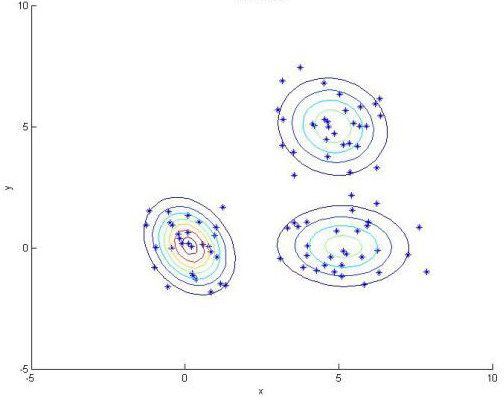
\includegraphics[scale=0.5]{Figures/gmm_example.png}
	\caption{Example of clustering using Gaussian Mixture Model}
	\label{fig:gmm_example}
\end{figure}
\end{comment}

\noindent It is important to note that in speaking recognition, it is allowed to assume that size of the acoustic space of the spectral. The spectral is referred to the phonetic events as we described in \ref{ch:english_language}. In fact, these acoustic classes have well defined features that allows the model to distinguish one phoneme from another. For the same reason, GMM is also used in \textit{speaker recognition} in which the vocal tracts spectral is taken into account to distinguish a speaker from another \cite{reynolds1992gaussian}. \\

\noindent Continuing with the speaker recognition example, we can think of the spectral shape $i$ as an acoustic class in which can be represented by the mean $\mu_{i}$ of the $i-th$ component density. The variation in the spectrum can be defined as the covariance matrix $\Sigma_{i}$. Also, a GMM can be views as a Hidden Markov Model with a single state assuming that the feature vectors are independent as well as the observation density from the acoustic classes is a Gaussian mixture \cite{reynolds2000speaker} \cite{reynolds1995robust}.

